\chapter{Estado del Arte}

De los trabajos que existen en la actualidad, podemos mencionar tres que resultan de especial interés, cuyas metodologías se encuentran las siguientes:
\begin{itemize}
	\item Búsqueda de reglas locales para un autómata celular mediante el análisis estadístico de las observaciones de un fenómeno.
	\item Configuración de reglas locales para un autómata celular mediante el empleo de algoritmos evolutivos.
	\item Búsqueda de reglas locales para un autómata celular mediante el empleo de algoritmos evolutivos para satisfacer un patrón especifico.
\end{itemize}

Estos son algunos de los enfoques para emplear los autómatas celulares como herramienta para modelar fenómenos, que si bien tienen relación con este trabajo de tesis, no se conectan directamente con el.

\section{Cellular Automata Automatically Constructed from a Bioconvection Pattern}

Esta investigación \citep{kawaharada2016cellular} se centra en realizar el descubrimiento de las reglas de evolución para un autómata celular unidimensional, empleando métodos de análisis estadísticos para determinar estas reglas a partir de los datos observados de los patrones de bioconvección generados como resultado de la respuesta a una estimulación luminosa de un tipo de alga unicelular llamada Euglena gracilis. 
\\
El experimento consistió en iluminar por la parte de abajo de un contenedor anular conteniendo una suspensión de E. gracilis con una fuerte intensidad de luz. Los individuos al ser alcanzados por la luz sufren de fototaxis negativa, lo cual hace que se acumulen cerca de la superficie. Como la densidad del E. gracilis es mas pesada que el agua, las regiones ricas en Euglena se precipitan al fondo para conducir el flujo local. Estas interacciones entre los individuos y el flujo eventualmente forma patrones de bioconvección.
\\
El proceso lo realizan de la siguiente forma:

\begin{enumerate}
	\item Recopilación de imágenes de los patrones de bioconvección.
	\item Transformación de las imágenes recopiladas a escala de grises.
	\item Uso de filtros para la eliminación del ruido.
	\item Discretización de las imágenes en escala de grises.
	\item Se predetermina el número de estados para el sitio $k$ y se discretiza la información observada acorde a esto.
	\item Basado en el número de vecinos establecido $m$ se calcula la frecuencia con la que aparecen los estados por cada combinación de posibles estados vecinos.
	\item Con base en esta frecuencia se determinan las reglas locales para el AC.
\end{enumerate}

\section{Discovery of Transition Rules for Cellular Automata Using Artificial Bee Colony and Particle Swarm Optimization Algorithms in Urban Growth Modeling}

En este trabajo \citep{naghibi2016discovery} se muestra un método para descubrir las reglas de transición de un autómata celular de lattice bidimensional que modele el crecimiento urbano empleando un algoritmo de optimización de colonia de abejas artificiales. Para ello utilizan como datos de entrada información multitemporal sensada remotamente de el área urbana de la ciudad de Urmia, Iran.
\\
El autómata celular en este trabajo se define con la siguiente ecuación:

\begin{equation} \label{eq:8}
P^t_{ij} = S^t_{ij}\times\Omega^t_{ij}\times Con\times e_r
\end{equation}
donde:
\begin{itemize}
	\item $P^t_{ij} $ es el potencial de desarrollo de una celda $ij$.
	\item $S^t_{ij}$ es la idoneidad de la celda $ij$ para cambiar basada en factores relevantes en el tiempo $t$.
	\item $\Omega^t_{ij}$ es el efecto que tiene la densidad de desarrollo del vecindario.
	\item $Con$ es una condición funcional que se vuelve verdadero cuando se encuentra la idoneidad de la celda.
	\item $e_r$ es un termino para la perturbación estocástica por errores.
\end{itemize}

El potencial de desarrollo se compara con un valor umbral para determinar si una célula no urbanizada va a poder ser transformada en una célula urbanizada en el tiempo $t+1$. Entonces los valores a encontrar son los valores de umbral para los cuales transiciona una célula no urbanizada a una urbanizada.
\\
Como requerimiento para la evaluación del algoritmo, se emplean otras dos técnicas además de la colonia de abejas artificiales,las cuales son:
\begin{itemize}
	\item Particle Swarm Optimization (PSO)
	\item Logistic Regression
\end{itemize}

Los siguientes diagramas de continuación muestran el procedimiento que se siguió con cada uno de los algoritmos para la calibración de las reglas para el autómata celular.

\begin{figure}[H]
	\centering
	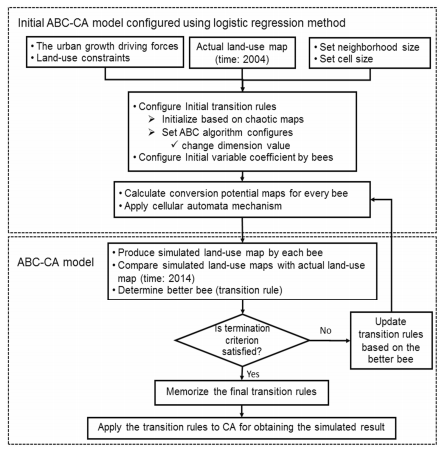
\includegraphics[width=\linewidth]{fig/abc}
	\caption{Modelo para la obtención de reglas del autómata celular empleando un algoritmo de optimización de colonia de abejas artificiales.}
	\label{fig:abc}
\end{figure}

\begin{figure}[H]
	\centering
	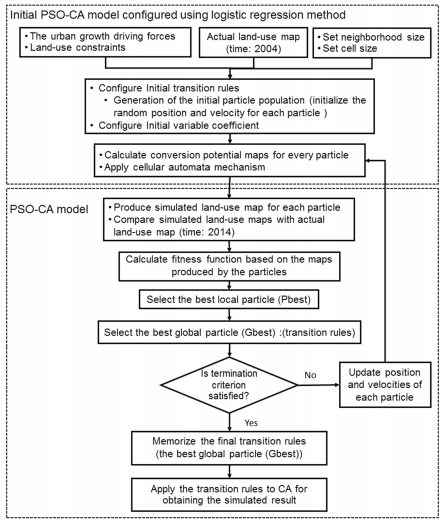
\includegraphics[width=\linewidth]{fig/pso}
	\caption{Modelo para la obtención de reglas del autómata celular empleando un algoritmo de optimización de enjambre de partículas.}
	\label{fig:pso}
\end{figure}

\begin{figure}[H]
	\centering
	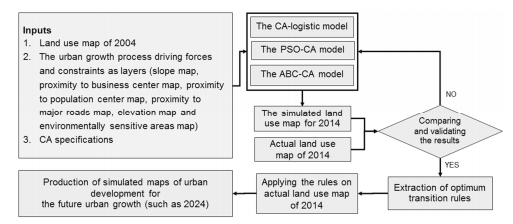
\includegraphics[width=\linewidth]{fig/evaluation}
	\caption{Modelo de evaluación de los algoritmos.}
	\label{fig:evaluation}
\end{figure}

\begin{figure}[H]
	\centering
	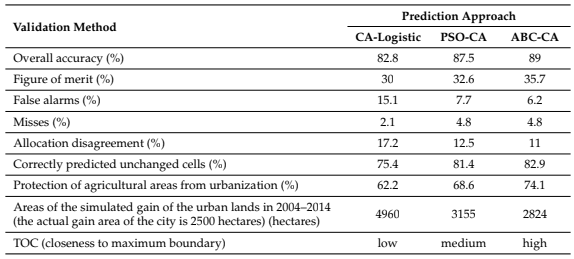
\includegraphics[width=\linewidth]{fig/results}
	\caption{Resultados de la evaluación de los algoritmos. }
	\label{fig:results}
\end{figure}

Como podemos ver en la tabla de resultados el algoritmo de colonia de abejas fue capaz de obtener un mejor rendimiento sobre los otros métodos, lo cual ayudara a obtener un mejor despeño para la estimación correcta del crecimiento urbano. Sin embargo este método aquí planteado sigue teniendo ciertos obstáculos como lo es encontrar la definición correcta de la ecuación que define al autómata celular.

\section{On Routine Evolution of Complex Cellular Automata}

El enfoque de este trabajo \citep{bidlo2016routine} es la creación de un método para la obtención de un conjunto de reglas que puedan replicar un comportamiento, sin embargo no toman en cuenta conocimiento previo del fenómeno que se quiere replicar. Lo que se hace es utilizar un algoritmo evolutivo cuya función de aptitud es dependiente del resultado al que se quiere llegar y la codificación de las reglas viene dada de la siguiente forma:

\begin{figure}[H]
	\centering
	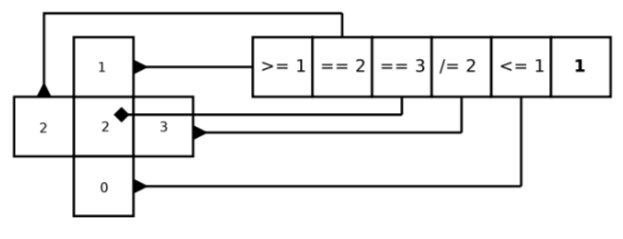
\includegraphics[width=\linewidth]{fig/rulesencoding}
	\caption{Ejemplo de la codificación de las reglas de evolución del autómata con un vecindario de tipo Moore.}
	\label{fig:rulesencoding}
\end{figure}
